\section{Indlæggelsesforløb og Personlige Omkostninger}
Indlæggelsesforløbene for apopleksipatienter varierer både i antal og hyppighed afhængig af forskellige faktorer - herunder alder og køn.

\subsection{Indlæggelsesforløb}
I 2010 var der i Danmark 18.041 indlæggelsesforløb forbundet med hjerneskade. Indlæggelsesforløbene kan inddeles i seks kategorier: Spontan blødning i hjernen, spontan infarkt i hjernen, uspecificeret apopleksi, diverse apopleksitilfælde, sequelae og TCI. \fxnote{Ydermere er forløbet for alle apopleksitilfælde inddelt i gruppe for sig selv, dette vil sige alle foruden sequelae og TCI.} Den hyppigste diagnose iblandt apopleksitilfælde var i 2010 spontan infarkt i hjernen med 6832 indlæggelsesforløb, hvilket svarer til omkring 38\% af alle forløbene. Den næsthyppigste var TCI som stod for omkring 27 \% af forløbene, hvor den laveste andel af indlæggelsesforløb, kaldet diverse, står for 0,8\% af det samlede antal. \fxnote{tænkte at vi kunne lave en tabel over de forskellige antal og sige at for yderligere kan ses i appendix, ellers kan vi sætte den ind} Indlæggelsesforløbene for apopleksi (ekslusiv sequale) er faldet siden år 2000, hvilket kan ses på \figref{Indlaeggelser}.[1]

\begin{figure}[H]
	\caption{Indlæggelsesforløb for apopleksi}
	\label{Indlaeggelser}
	\centering
	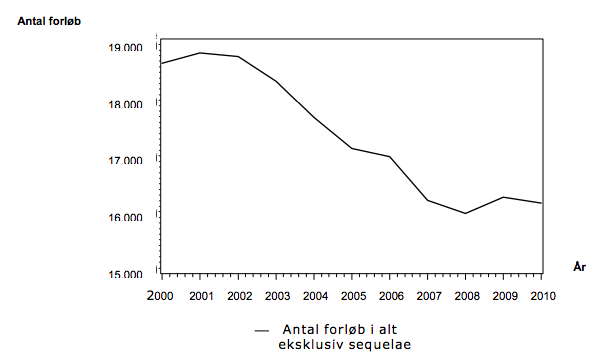
\includegraphics[scale=.5]{figures/bProblemanalyse/Figur1}
	\flushleft
	\textit{Her illustreres faldet i antallet af indlæggelsesforløb siden 2000.}
\end{figure}

Indlæggelsesforløbene har forskellig længde. 16.460 forløb, og dermed størstedelen, varede under 15 dage. For perioden fra 15-28 dage var der 1.191 forløb. Efter dette var tallet støt faldende, med kun 3 indlæggelsesforløb der er over 150 dage [1].

\subsection{Køn- og aldersfordeling}
Hvis der ses på fordelingen af køn og aldersgrupper der rammes af apopleksi, stod mændene i 2010 for 9.710 af alle tilfælde, mens kvinderne stod for 8.562 [1]. Dette svarer til at mændene stod for 53\% af alle tilfældene[3]. Fordelingen kan ses på \figref{AlderKoen}.  
Antallet af indlæggelsesforløb for mænd stiger, når de bliver ældre end 65 år. Dette ses også på \figref{AlderKoen}, der viser at der i 2010 næsten skete en fordobling i gruppen 65+ i forhold til gruppen under 65.
Kvinders antal af indlæggelsesforløb fulgte samme mønster som mændene, og steg til over det dobbelte ved gruppen 65+ i forhold til gruppen under 65, som pgså er illustreret på \figref{AlderKoen}.[1] Alderen er således en væsentlig faktor for forekomsten af apopleksi.

\begin{figure}[H]
	\caption{Alders- og kønsfordeling}
	\label{AlderKoen}
	\centering
	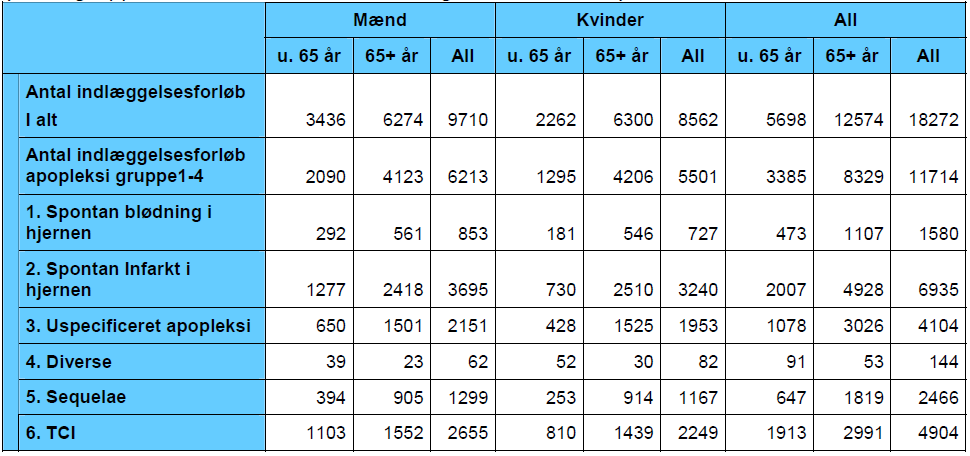
\includegraphics[scale=.8]{figures/bProblemanalyse/MaendKvinder}
	\flushleft
	\textit{Tabellen viser fordelingen af apopleksipatienter i forhold til alder og køn i 2010.}
\end{figure}

\subsection{Fremtidsprognoser}
Patienterne kan, som tidligere nævnt, rammes af en række følger som både kan have indflydelse på det fysiske og mentale. Ud fra alle tilfælde af apopleksi levede 75.000 over 18 i år 2011 med følger efter et slagstilfælde[3]. Dette tal forventes at være stigende i takt med at der kommer flere ældre [4]. Antallet der dør af hjerneskader har været stagneret de sidste 10 år før 2011, hvor 14 \% døde inden for 30 dage[3]. Det vil derfor kunne forventes, at der er flere, som kommer ud for en hjerneskade og vil have mén herefter, hvilket gør det vigtigt at fokusere på rehabiliteringen for at kunne genoptræne de forskellige kropslige og mentale mangler.

\section{Livskvalitet}
Dette afsnit er baseret på hjerneskader generelt. Dvs. det ikke er sikkert, at apopleksi er årsagen, men det antages, at de samme udfordringer gør sig gældende hos personer, der får hjerneskader af apopleksi. Derudover skal det noteres, at det ikke er sikkert, at en apopleksiramt får en hjerneskade. 

Personer der første gang rammes af en hjerneskade, beskriver hjerneskaden som et brud i deres liv, som de skal lære at forholde sig til. Derudover kan det tage lang tid for patienterne at indse, at de er ramt af en sygdom. 
Hjerneskaden går ind og influerer den ramtes humør, personlighed, færdigheder, aktiviteter, samt sociale relationer. Ud fra de ovennævnte skader påvirkes patienterne af  en uvished og usikkerhed, som patienterne kan risikere at leve med i lang tid, afhængigt af hvilken grad hjerneskaden har haft.[2] 

\subsection{Identitet}
En hjerneskadets identitet ændres, da patienten ikke er i stand til at udføre de samme opgaver som tidligere. Derfor bliver den hjerneskadede nødt til at skabe en ny identitet, hvilket for mange kan være svært. Kroppens funktionsændringer gør, at den ramte kommer til at leve et mere inaktivt og hjemmeorienteret liv end før. En yngre patient er mere ramt af denne forandring i forhold til en ældre patient. Apopleksiramte kan derudover opleve en kropsspaltning, hvor kroppen opleves som et fremmet objekt. Et objekt, som kan være svært at styre og ikke gør, som patienten vil.[2] 

Der findes skjulte vanskeligheder for patienter med hjerneskade. Disse omfatter vanskelighed med hukommelse, læsning, regning samt andre færdigheder, der ikke er let synlige. Disse skjulte vanskeligheder har også en indflydelse på, hvordan patienten opfatter sig selv og kan være med til at nedsætte livskvaliteten for den enkelte.[2] 

\subsection{Patienternes påvirkning}
Alle de fysiske og mentale ændringer medfører, at det er svært for en hjerneskadet patient at vende tilbage til sit gamle hverdagsliv. Forandringerne gør det svært at udføre almindelige huslige pligter, såsom rengøring og personlig pleje. De ramte oplever det også som en svær oplevelse at vende tilbage på arbejde. Dette skyldes, udover de kropslige og mentale ændringer, også den træthed, der kan opleves. Det er derfor vigtigt at føle sig værdsat på jobbet. Den hjerneskadede patient skal vende tilbage til sine sociale relationer. Dette kan opleves som en meget hård opgave pga. de forandringer, kroppen har gennemgået. Det ses imidlertid, at familierelationerne bliver tættere, mens relationerne til vennerne bliver mindre. Dette er et problem, da gode relationer kan være med til at forbedre rehabiliteringsprocessen og dermed gøre, at den hjerneskadede patient hurtigere kan komme tilbage til et normalt liv. [2]

Ud fra  det ovenstående kan det konkluderes, at hjerneskadede patienter, heriblandt apopleksiramte, oplever nedsat livskvalitet pga. deres sygdom. Dette kan også ses ved, at apopleksipatienter har dobbelt så stor selvmordsrate som baggrundsbefolkningen. Derudover nævner 16\% af apopleksi patienter, at deres livskvalitet er dårlig, 46\% syntes den er nogenlunde, mens 38\% synes den er god. Den nedsatte livskvalitet er noget der kan føre til vanskeligheder senere i livet, hvilket selvfølgelig skal forsøges undgået. En forbedret livskvalitet kan skabes ved hurtigere rehabilitering eller forbedret kropslig funktion, som den apopleksiramte patient mistede ved hjerneskaden. [2]  


[1] - Beskrivelse af dataopgørelse for voksne med apopleksi og TCI med tabeller og grafik. 
[2] - Hjerneskaderehabilitering, Sundhedsstyrelsen
[3] - Hjertesagen.dk
[4] - aeldresagen

%Det ses her, at mænd står for 9.710 af apopleksi tilfælde, mens kvinderne står for 8.562 [1]. For mændene er 3.436 af tilfældene udgjort af personer under 65 år, mens 6.274 af tilfældene finder sted for personer over 65 år [1]. For kvinderne står personerne over 65 år for 6.300 af tilfældene, mens dem under 65 år står for 2.262 af tilfældene [1]. Det ses ud fra dette, at mænd og kvinder bliver ramt af apopleksi på lige fod, altså er apopleksi et lige stort problem for kvinder som det er for mænd.
% Spontan blødning i hjernen, stod for 1547 af tilfældene; Apopleksi: Spontan infarkt i hjernen, stod for 6832 af tilfældene; Uspecificeret apopleksi, stod for 4049 af tilfældene; diverse, stod for 141 af tilfældene; Sequelae, stod for 2450 af tilfældene; TCI, stod for 4860 af tilfældene [1]. Sequelae tilfældene er ikke nødvendigvis et apopleksi tilfælde, men en anden sygdom der forekom på grund af apopleksi [1]. 
%Selve aldersfordelingen af personer som rammes af apopleksi, fordeler sig forholdsvis ens hos både mænd og kvinder. Den største andel ses for begge køn for personer over 65 år, hvilket svarer til 65 \% for mænd og  73 \% for kvinder. Ud af dette kan det konkluderes at der sker 8\% flere tilfælde af apopleski for mænd end kvinder.
%Aldersfordelingen er for begge køn et overtal af personer over 65 år, det ses dog at der er flere kvinder der rammes i en alder over 65 år. % Kan man lave en graf på dette? 